\documentclass[
  10pt,
  twocolumn,
  aps,
  pra,
  showkeys,
  amsmath,amssymb,
  longbibliography
]{revtex4-2}

\usepackage[T1]{fontenc}
\usepackage[utf8]{inputenc}
\usepackage{mathptmx}
\usepackage{amsthm}
\usepackage{graphicx}
\usepackage{booktabs}
\usepackage{xcolor}
\usepackage{array}
\usepackage{tikz}
\usetikzlibrary{calc,matrix,positioning}
\usepackage{listings}
\lstset{language=Prolog, basicstyle=\footnotesize\ttfamily,
  columns=fullflexible, keepspaces=true, showstringspaces=false,
  breaklines=true, frame=tb, framesep=4pt,
  aboveskip=5pt, belowskip=5pt}
\usepackage[
  breaklinks=true,
  colorlinks=true,
  citecolor=blue,
  linkcolor=blue,
  urlcolor=blue
]{hyperref}
\usepackage{orcidlink}


\newtheorem{proposition}{Proposition}

% --- Colors for states ---
\definecolor{stateone}{HTML}{3A9D5D}   % green
\definecolor{statetwo}{HTML}{3C74C6}   % blue
\definecolor{statethree}{HTML}{C84332} % red
\definecolor{statefour}{HTML}{D8922C}  % orange
\definecolor{statefive}{HTML}{7C52B8}  % violet
\definecolor{lightfalse}{HTML}{E6E6E6}

% --- TikZ tiles for figures ---
\tikzset{
  qtile/.style={draw=black, minimum width=4.2mm, minimum height=4.2mm, inner sep=0pt},
  tileone/.style={qtile, fill=stateone},
  tiletwo/.style={qtile, fill=statetwo},
  tilethree/.style={qtile, fill=statethree},
  tilefour/.style={qtile, fill=statefour},
  tilefive/.style={qtile, fill=statefive},
  tilefalse/.style={qtile, fill=lightfalse, draw=gray!70},
  tilesep/.style={qtile, fill=black},
  tileblank/.style={qtile, fill=white, draw=gray!30}
}

% --- Simple listing replacement ---
\newcounter{listing}
\renewcommand{\thelisting}{\arabic{listing}}

\newcommand{\listingtitle}[2]{%
  \refstepcounter{listing}%
  \par\smallskip
  \noindent\textbf{Listing \thelisting.} #2%
  \label{#1}%
  \par\smallskip
}

\begin{document}

\title{Quantum Structures as Generative Scores:\texorpdfstring{\\}{ }
Partition Logic, Generative Logic, and Aesthetic Form}
\hypersetup{pdftitle={Quantum Structures as Generative Scores: Partition Logic, Generative Logic, and Aesthetic Form},
  pdfauthor={Christian Jendreiko and Karl Svozil}}

\author{Christian Jendreiko\,\orcidlink{0009-0006-4302-6261}}
\affiliation{HSD University of Applied Sciences, M\"unsterstra{\ss}e 156, D-40476 D\"usseldorf, Germany}
\email{christian.jendreiko@hs-duesseldorf.de}
\author{Karl Svozil\,\orcidlink{0000-0001-6554-2802}}
\affiliation{Institute for Theoretical Physics, TU Wien, Wiedner Hauptstrasse 8-10/136, A-1040 Vienna, Austria}
\email{karl.svozil@tuwien.ac.at}

\date{\today}

\begin{abstract}
We connect partition logic with Generative Logic by translating finite partition logics into Prolog-based Simple Generative Logic Grammars. As a proof of concept, we use the five-atom V-logic \(L_{12}\) to generate a modular visual artifact, the \emph{Quantum Square}. The approach separates logical structure from its visual, textual, or sonic realization. The examples establish a generative design method and suggest a way to introduce contexts and complementarity through perceptible form.
\end{abstract}

\keywords{partition logics, logic programming, quantum structures, quantum music, generative logic, complementarity, generative art, generative design, science communication, Prolog, education}

\maketitle

\section{Introduction}

This paper connects two lines of work that are rarely discussed together. One originates in the logical and combinatorial study of finite empirical structures in quantum foundations, especially partition logics and related event structures \cite{svozil-93,schaller-92,dvur-pul-svo,svozil-ql,svozil-2001-eua}. The other originates in artistic research and design education, namely Christian Jendreiko's concept of \emph{Generative Logic} and the associated \emph{Simple Generative Logic Grammar} (SGLG), which treats Prolog as a generative engine for aesthetic production \cite{Jendreiko2024,Jendreiko2025}.

The shared premise is that formal structures are not only objects of abstract analysis; they can also act as structuring agents. In mathematics, this idea is familiar from fractals, cellular automata, L-systems, symmetry groups, and stochastic processes. In design, one encounters related practices whenever a rule system is used to generate, constrain, or organize visual, textual, or sonic material. The present paper asks whether partition logics can be used in this way: not merely as representations of finite event structures, but as engines for the generation of perceptible artifacts.

This question has both an aesthetic and a communicative side. Finite logical structures exhibit repetition, asymmetry, recurrence, and nontrivial forms of overlap. These can become aesthetically productive once mapped into color, shape, spacing, rhythm, or timbre. At the same time, concepts such as context, complementarity, and non-Boolean composition are often difficult to grasp when they remain purely symbolic. If they can be externalized into visual or sonic form without losing their structural discipline, they may become more accessible.

The key methodological move of the paper is the separation of three layers:
\begin{enumerate}
\item a \emph{formal skeleton}, given by a partition logic or related finite event structure;
\item a \emph{generative grammar}, which translates that skeleton into a structured template of positions;
\item a \emph{sign repertoire and rendering rule}, which realizes that structure in a concrete medium.
\end{enumerate}
This separation is important both artistically and scientifically. Artistically, it allows the same structure to migrate across media. Scientifically, it prevents us from conflating a combinatorial structure with a particular physical realization or probability theory.

The paper does four things. First, it gives a compact account of the partition-logical source structures used here. Second, it states a general translation from finite partition logics with separating sets of two-valued states into SGLGs. Third, it develops a proof of concept: the V-logic \(L_{12}\) is translated into a visual artifact, the \emph{Quantum Square}. Fourth, it extends the method to a triangle logic and discusses the resulting structures from the perspectives of design and science communication.

\section{Partition logic between formal structure and design material}

\subsection{Partitions and partition logics}

Let \(\Omega_n=\{1,2,\dots,n\}\) be a finite set. A \emph{partition} \(\pi\) of \(\Omega_n\) is a family of nonempty, pairwise disjoint subsets whose union is \(\Omega_n\). The elements of a partition are its \emph{blocks}. Each partition can be identified with the atoms of a finite Boolean algebra. A \emph{partition logic} is obtained by selecting several such Boolean algebras and pasting them together through identified common elements \cite{schaller-92,dvur-pul-svo,svozil-2001-eua}.

In the language of quantum logic, the pasted Boolean algebras are often called \emph{contexts}. They provide local classical views within a structure that may be non-Boolean. Here, complementarity means that no single available context jointly resolves the distinctions offered by the different contexts. Although partitions of the same set always have a common set-theoretic refinement, that refinement need not be an available measurement. The distinction is therefore between what exists in the underlying state space and what can be resolved within the chosen empirical structure.

Partition logics are therefore well suited to interdisciplinary transfer. They are finite, explicit, and combinatorial. At the same time, they already carry key motifs associated with quantum theory: contextual decomposition, overlap of contexts, and non-Boolean composition.

\subsection{Formal Example A: a horizontal sum of binary partitions}

A minimal example uses the set
\begin{equation}
\Omega_3=\{1,2,3\}.
\end{equation}
Consider the three binary partitions
\begin{align}
\pi_1 &= \{\{1\},\{2,3\}\},
\nonumber\\
\pi_2 &= \{\{2\},\{1,3\}\},
\nonumber\\
\pi_3 &= \{\{3\},\{1,2\}\}.
\label{eq:threepartitions}
\end{align}
If these three Boolean algebras are pasted only in their bottom and top elements, one obtains a horizontal sum of three four-element Boolean algebras. This is a simple non-Boolean event structure.

To make the example more readable, let us name the six atoms
\begin{align}
p &\leftrightarrow \{1\}, & \neg p &\leftrightarrow \{2,3\},
\nonumber\\
q &\leftrightarrow \{2\}, & \neg q &\leftrightarrow \{1,3\},
\nonumber\\
r &\leftrightarrow \{3\}, & \neg r &\leftrightarrow \{1,2\}.
\end{align}
A \emph{two-valued state} assigns each atom either \(0\) or \(1\), with exactly one atom assigned \(1\) in each context. A family of states is \emph{separating} if any two distinct propositions receive different values in at least one state. The underlying points \(1,2,3\) induce three such states \(s_1,s_2,s_3\). They form a separating selection from the eight two-valued states of the abstract horizontal sum; we use this selection for the example. The supports are then
\begin{align}
T(p)&=\{s_1\}, & T(\neg p)&=\{s_2,s_3\},
\nonumber\\
T(q)&=\{s_2\}, & T(\neg q)&=\{s_1,s_3\},
\nonumber\\
T(r)&=\{s_3\}, & T(\neg r)&=\{s_1,s_2\}.
\label{eq:hsupports}
\end{align}
Even this small logic shows a pattern that later becomes generative: the same finite set of state symbols is redistributed from context to context.

\subsection{Formal Example B: the V-logic \texorpdfstring{\(L_{12}\)}{L12}}

Our main proof of concept uses the five-atom V-logic \(L_{12}\), consisting of two three-atomic contexts
\begin{equation}
C_1=\{a,b,c\},
\qquad
C_2=\{c,d,e\},
\end{equation}
with intertwining atom \(c\). Figure~\ref{fig:vlogic}(a) shows the corresponding 3-uniform hypergraph in Greechie-style notation \cite{greechie:71}, in which contexts are represented schematically by unbroken lines that intersect at shared atoms.

This logic has exactly five two-valued states, shown in Table~\ref{tab:vstates}. They separate the atoms and therefore provide a classical state space for a partition-logical representation \cite[Theorem~0]{kochen1}.

\begin{table}[b]
\caption{The five two-valued states of the V-logic \(L_{12}\).}
\label{tab:vstates}
\begin{ruledtabular}
\begin{tabular}{c c c c c c}
state & \(a\) & \(b\) & \(c\) & \(d\) & \(e\) \\
\hline
\(s_1\) & 1 & 0 & 0 & 0 & 1 \\
\(s_2\) & 1 & 0 & 0 & 1 & 0 \\
\(s_3\) & 0 & 1 & 0 & 0 & 1 \\
\(s_4\) & 0 & 1 & 0 & 1 & 0 \\
\(s_5\) & 0 & 0 & 1 & 0 & 0 \\
\end{tabular}
\end{ruledtabular}
\end{table}

The supports of the atoms are
\begin{align}
T(a)&=\{s_1,s_2\}, & T(b)&=\{s_3,s_4\}, & T(c)&=\{s_5\},
\nonumber\\
T(d)&=\{s_2,s_4\}, & T(e)&=\{s_1,s_3\}.
\label{eq:vlogic_supports}
\end{align}
Equivalently, by identifying each atom with the set of two-valued states in which it is assigned the value \(1\) \cite{svozil-2001-eua}, the two contexts are represented by the partitions
\begin{equation}
\begin{split}
&\{\{s_1,s_2\},\{s_3,s_4\},\{s_5\}\},
\;
\{\{s_5\},\{s_2,s_4\},\{s_1,s_3\}\};
\\
&\text{or, equivalently,}
\\
&\{\{1,2\},\{3,4\},\{5\}\},
\;
\{\{5\},\{2,4\},\{1,3\}\}.
\end{split}
\end{equation}

The conceptual importance of this example, as well as the previous example involving horizontal sums, is that it exhibits complementarity while still possessing a separating set of two-valued states. Thus it does \emph{not} exhibit Kochen-Specker-type value indefiniteness \cite{kochen1}. For science communication this is advantageous: it allows one to explain context dependence without prematurely introducing stronger no-go results.

\subsection{A quantum realization of the same logical form}

The same V-logic also admits a faithful orthogonal representation \cite{lovasz-79,GroetschelLovaszSchrijver1986} in three-dimensional Hilbert space. A simple choice is
\begin{equation}
\begin{split}
&|a\rangle = (1,0,0)^{\mathsf T},
\quad
|b\rangle = (0,1,0)^{\mathsf T},
\\
&|c\rangle = (0,0,1)^{\mathsf T},
\\
&|d\rangle = (\cos\theta,\sin\theta,0)^{\mathsf T},
\quad
|e\rangle = (-\sin\theta,\cos\theta,0)^{\mathsf T},
\label{eq:hilbertrealization}
\end{split}
\end{equation}
with \(0<\theta<\pi/2\).
Then \(\{|a\rangle,|b\rangle,|c\rangle\}\) and \(\{|c\rangle,|d\rangle,|e\rangle\}\) form two orthonormal bases sharing the ray \(c\). Neither \(|a\rangle\) nor \(|b\rangle\) is orthogonal to \(|d\rangle\) or \(|e\rangle\).

The V-logic thus provides both a partition representation and a quantum realization. The latter also requires geometric information, here the angle \(\theta\), that the logical skeleton alone does not specify. The grammars below use the two-valued-state supports and introduce no probabilistic weighting.

\section{Generative Logic and SGLGs}

\subsection{Generative Logic}

Generative Logic, introduced in Refs.~\cite{Jendreiko2024,Jendreiko2025}, treats Prolog not only as a language for symbolic computation but as a generative environment in which rules, substitutions, and derivations become design operations. The Prolog inference engine functions as a disciplined producer of variants. In this perspective, the logical formula is not only a specification of truth conditions; it is also a compositional device.

This is particularly relevant in artistic research and education. It allows students and researchers to work with rule systems that remain both transparent and executable. The output need not remain verbal or symbolic. Once a derivation is mapped into color, sound, or spatial arrangement, a logical process becomes a perceptible artifact.

\subsection{A Simple Generative Logic Grammar}

To turn a partition logic into an executable generative scheme, we use a Simple Generative Logic Grammar (SGLG) \cite{Jendreiko2025}. In the present paper, this grammar is understood in a practical way: it specifies how a finite artifact is assembled from rows and symbols, while a separate rendering map determines how those symbols appear in a given medium.

We write the grammar as
\begin{equation}
G=(\mathcal N,\Sigma,P,S,M,\Lambda),
\end{equation}
where \(\mathcal N\) is a set of nonterminal symbols, \(\Sigma\) is a set of state symbols, \(P\) is a set of production rules, \(S\) is the start symbol, and \(\Lambda\) contains layout symbols such as separators and line breaks. Productions expand nonterminals into sequences over \(\mathcal N\cup\Sigma\cup\Lambda\), while \(M\) assigns concrete realizations to the terminal and layout symbols.

For the present purposes, a production rule of the form
\begin{equation}
\texttt{Head -{}-> Body}
\end{equation}
may be read simply as an assembly rule: the head is expanded into the ordered sequence given by the body. For example, if the complete artifact consists of five rows, one may write
\begin{equation}
q_L \to a\,b\,c\,d\,e
\end{equation}
meaning that the whole object is built from the rows \(a,b,c,d,e\). A row may then be specified by a rule such as
\begin{equation}
a \to s_1\,s_2\,br\,s_3\,s_4\,s_5\,n
\end{equation}
where \(s_1,\dots,s_5\) are state symbols, \(br\) is a separator, and \(n\) denotes a line break.

The grammar therefore determines the structure of the output, but not yet its concrete appearance. The rendering map \(M\) assigns a medium-specific realization to each symbol. For instance, one may choose
\begin{equation}
s_1 \mapsto \text{green square},
\qquad
s_2 \mapsto \text{blue square}
\end{equation}
and similarly for the other symbols. By changing \(M\), the same grammar can be realized visually, textually, or sonically.

In Jendreiko's broader framework, such rules may also be interpreted as containment relations, in that larger forms contain the smaller ones they are composed of.

The non-recursive character of the grammar is important here. It guarantees that every derivation terminates after finitely many steps and yields a finite, inspectable artifact.

\section{From partition logic to grammar}

The preceding grammar scheme becomes concrete once its symbols are taken from a partition logic. The basic idea is simple: atoms of the logic become row labels, two-valued states become recurring symbols, and a separator divides the states that make a given atom true from those that make it false.

Let \(L\) be a finite partition logic with atoms
\begin{equation}
A=\{x_1,\dots,x_m\}
\end{equation}
and a separating set of two-valued states
\begin{equation}
V_L=\{v_1,\dots,v_N\}.
\end{equation}
Associate a symbol \(s_i\) with each two-valued state \(v_i\), and write
\begin{equation}
\mathcal{S}_N=\{s_1,\dots,s_N\}.
\end{equation}
For each atom \(x_j\), define
\begin{equation}
T(x_j)=\{s_i\in\mathcal{S}_N \mid v_i(x_j)=1\},
\qquad
F(x_j)=\mathcal{S}_N\setminus T(x_j).
\label{eq:tfsets}
\end{equation}
Thus \(T(x_j)\) is the set of state symbols for which \(x_j\) is true, and \(F(x_j)\) is the complementary set for which \(x_j\) is false. Fix an order of the atoms and of the states. In a production rule, \(T(x_j)\) and \(F(x_j)\) denote lists in the induced state order; the examples use increasing indices.

We then construct a grammar \(G_L\) with start symbol \(q_L\) by setting
\begin{align}
q_L &\to x_1\,x_2\,\cdots\,x_m,
\label{eq:startrule2}
\\
x_j &\to T(x_j)\,br\,F(x_j)\,n.
\label{eq:rowrule2}
\end{align}
Here \(br\) is a separator symbol and \(n\) is a layout symbol such as a line break. In words: the whole artifact consists of one row for each atom, and the row of \(x_j\) lists first those states in which \(x_j\) is true and then those in which it is false.

\begin{proposition}
Let \(L\) be a finite partition logic with separating two-valued states. The grammar \(G_L\) constructed from Eqs.~\eqref{eq:tfsets}--\eqref{eq:rowrule2} preserves the incidence relation between atoms and two-valued states. In the generated row for \(x_j\), the symbol \(s_i\) occurs to the left of the separator iff \(v_i(x_j)=1\), and to the right iff \(v_i(x_j)=0\).
\end{proposition}

\begin{proof}
The two lists partition the state symbols according to the value of \(v_i(x_j)\), and the row rule places them on opposite sides of the separator. Concatenating all rows retains this information for every atom.
\end{proof}

The translation preserves atom--state incidence for the selected state family; the designated contexts remain part of the source specification and are not separately encoded in the rows. To recover the incidence from a rendering, the state symbols, separator, and row boundaries must remain distinguishable. Choosing a different separating family or ordering can change the artifact, so these choices belong to the score.

The construction is easiest to understand through examples.

\subsection{Formal Example C: the horizontal sum as a grammar}

Applying the translation to the horizontal-sum example of Eq.~\eqref{eq:threepartitions} yields
\begin{align}
p &\to s_1\,br\,s_2\,s_3\,n,
&
\neg p &\to s_2\,s_3\,br\,s_1\,n,
\nonumber\\
q &\to s_2\,br\,s_1\,s_3\,n,
&
\neg q &\to s_1\,s_3\,br\,s_2\,n,
\nonumber\\
r &\to s_3\,br\,s_1\,s_2\,n,
&
\neg r &\to s_1\,s_2\,br\,s_3\,n.
\label{eq:horizontalgrammar}
\end{align}
Each row corresponds to one atom, and the recurring symbols \(s_1,s_2,s_3\) record which of the three selected two-valued states support that atom. Even in this small example, the grammar already produces a visible pattern of repetition and redistribution.

\subsection{Formal Example D: the V-logic as a grammar}

The V-logic \(L_{12}\) is handled in exactly the same way. Since it has five atoms and five two-valued states, the resulting artifact has five rows built from the recurring symbols \(s_1,\dots,s_5\). Using the supports listed in Eq.~\eqref{eq:vlogic_supports}, we obtain
\begin{align}
a &\to s_1\,s_2\,br\,s_3\,s_4\,s_5\,n,
\nonumber\\
b &\to s_3\,s_4\,br\,s_1\,s_2\,s_5\,n,
\nonumber\\
c &\to s_5\,br\,s_1\,s_2\,s_3\,s_4\,n,
\nonumber\\
d &\to s_2\,s_4\,br\,s_1\,s_3\,s_5\,n,
\nonumber\\
e &\to s_1\,s_3\,br\,s_2\,s_4\,s_5\,n.
\label{eq:vgrammar}
\end{align}
This is the structural core of the \emph{Quantum Square}. The grammar fixes the arrangement of symbols row by row, beginning with the start rule as the point of entry for the generation:
\begin{equation}
q_L \to a\,b\,c\,d\,e.
\end{equation}

To obtain a visual realization, we map the five state symbols to five squares of identical size with five colors:
\begin{align}
s_1 &\mapsto \text{green},
&
s_2 &\mapsto \text{blue},
&
s_3 &\mapsto \text{red},
\nonumber\\
s_4 &\mapsto \text{orange},
&
s_5 &\mapsto \text{violet}.
\label{eq:vpalette}
\end{align}
The separator \(br\) is rendered as a black square. The name \emph{Quantum Square} refers to the artwork; with separators included, the displayed arrangement has five rows and six columns.

The supports determine which symbols lie on each side of the separator; the chosen ordering determines their sequence. The palette and tile geometry are rendering choices.



\section{The Quantum Square: structure and renderings}

Figure~\ref{fig:vlogic} connects the V-logic and its incidence schema with two renderings of the same grammar: colored tiles and a compact typographic arrangement.

\begin{figure*}[t]
\centering
\setlength{\tabcolsep}{3pt}
\begin{tabular}{cccc}
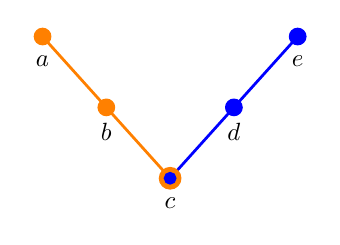
\begin{tikzpicture}[scale=0.90, transform shape, every path/.style={line width=1pt}]

% lines
\draw[orange] (0,2)--(0.9,1)--(1.8,0);
\draw[blue]   (1.8,0)--(2.7,1)--(3.6,2);

% orange context
\filldraw[fill=orange, draw=orange] (0,2) circle (3pt);
\node[yshift=-10pt] at (0,2) {$a$};

\filldraw[fill=orange, draw=orange] (0.9,1) circle (3pt);
\node[yshift=-10pt] at (0.9,1) {$b$};

% shared node c
\filldraw[fill=orange, draw=orange] (1.8,0) circle (4pt);
\filldraw[fill=blue,   draw=blue]   (1.8,0) circle (2pt);
\node[yshift=-10pt] at (1.8,0) {$c$};

% blue context
\filldraw[fill=blue, draw=blue] (2.7,1) circle (3pt);
\node[yshift=-10pt] at (2.7,1) {$d$};

\filldraw[fill=blue, draw=blue] (3.6,2) circle (3pt);
\node[yshift=-10pt] at (3.6,2) {$e$};

\end{tikzpicture}
&
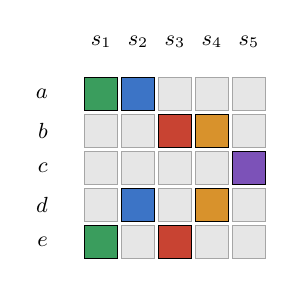
\begin{tikzpicture}[scale=0.88, transform shape]
\matrix (n) [matrix of nodes,
  nodes in empty cells,
  row sep=1pt,
  column sep=1pt,
  ampersand replacement=\&] {
|[tileone]| \& |[tiletwo]| \& |[tilefalse]| \& |[tilefalse]| \& |[tilefalse]| \\
|[tilefalse]| \& |[tilefalse]| \& |[tilethree]| \& |[tilefour]| \& |[tilefalse]| \\
|[tilefalse]| \& |[tilefalse]| \& |[tilefalse]| \& |[tilefalse]| \& |[tilefive]| \\
|[tilefalse]| \& |[tiletwo]| \& |[tilefalse]| \& |[tilefour]| \& |[tilefalse]| \\
|[tileone]| \& |[tilefalse]| \& |[tilethree]| \& |[tilefalse]| \& |[tilefalse]| \\
};
\node[left=4mm of n-1-1] {\small \(a\)};
\node[left=4mm of n-2-1] {\small \(b\)};
\node[left=4mm of n-3-1] {\small \(c\)};
\node[left=4mm of n-4-1] {\small \(d\)};
\node[left=4mm of n-5-1] {\small \(e\)};

\node[above=3mm of n-1-1] {\small \(s_1\)};
\node[above=3mm of n-1-2] {\small \(s_2\)};
\node[above=3mm of n-1-3] {\small \(s_3\)};
\node[above=3mm of n-1-4] {\small \(s_4\)};
\node[above=3mm of n-1-5] {\small \(s_5\)};
\end{tikzpicture}
&
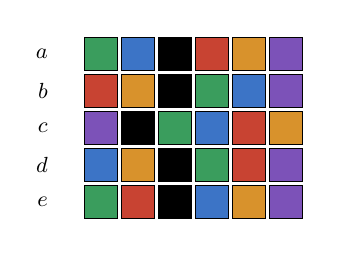
\begin{tikzpicture}[scale=0.88, transform shape]
\matrix (m) [matrix of nodes,
  nodes in empty cells,
  row sep=1pt,
  column sep=1pt,
  ampersand replacement=\&] {
|[tileone]| \& |[tiletwo]| \& |[tilesep]| \& |[tilethree]| \& |[tilefour]| \& |[tilefive]| \\
|[tilethree]| \& |[tilefour]| \& |[tilesep]| \& |[tileone]| \& |[tiletwo]| \& |[tilefive]| \\
|[tilefive]| \& |[tilesep]| \& |[tileone]| \& |[tiletwo]| \& |[tilethree]| \& |[tilefour]| \\
|[tiletwo]| \& |[tilefour]| \& |[tilesep]| \& |[tileone]| \& |[tilethree]| \& |[tilefive]| \\
|[tileone]| \& |[tilethree]| \& |[tilesep]| \& |[tiletwo]| \& |[tilefour]| \& |[tilefive]| \\
};
\node[left=4mm of m-1-1] {\small \(a\)};
\node[left=4mm of m-2-1] {\small \(b\)};
\node[left=4mm of m-3-1] {\small \(c\)};
\node[left=4mm of m-4-1] {\small \(d\)};
\node[left=4mm of m-5-1] {\small \(e\)};
\end{tikzpicture}
&
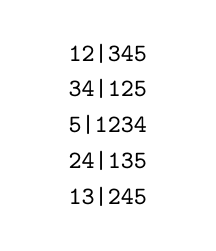
\begin{tikzpicture}[scale=0.88, transform shape]
\matrix [matrix of nodes,
  nodes={font=\ttfamily\small, minimum height=4.2mm,
    minimum width=18mm, inner sep=0pt},
  row sep=1pt] {
12|345\\
34|125\\
5|1234\\
24|135\\
13|245\\
};
\end{tikzpicture}
\\
(a) & (b) & (c) & (d)
\end{tabular}
\caption{The V-logic \(L_{12}\). (a) Greechie-style hypergraph. (b) Atom-state incidence schema, with colored cells indicating \(v_i(x)=1\) and gray cells indicating \(v_i(x)=0\). (c) The grammar-generated output, the \emph{Quantum Square}. In each row, the states assigning value \(1\) to the atom are listed first, then a black separator, and then the states assigning value \(0\). (d) The same rows rendered as digits, with \texttt{|} as separator.}
\label{fig:vlogic}
\end{figure*}

Panels~(c) and~(d) preserve the same incidence information while offering different perceptual cues: color emphasizes recurrence, whereas digits make symbol identity explicit. They also show the scope of the method: a fixed grammar produces one symbolic arrangement, while changes to its rendering yield different realizations.

\subsection{Why this object is aesthetically interesting}

The \emph{Quantum Square} is not a picture of a quantum system in any naive representational sense. It does not depict particles, trajectories, or apparatuses. Rather, it externalizes a formal relation as a visible organization of repetition and difference.

What becomes aesthetically salient is the disciplined reappearance of the same five colors across distinct rows, each row embodying a different logical perspective on the same finite state space. In design terms, this produces a tension between consistency and redistribution. In humanities terms, one may say that the logic functions as a score: it does not determine one unique expressive surface, but it constrains a field of possible realizations. In logical terms, it preserves the incidence of atoms and the selected states.

\section{A triangle-logic generalization of the Quantum Square}

To show that the method is not specific to the V-logic, we now apply it to the \emph{Wright triangle} \cite{dvur-pul-svo,wright}, represented by three partitions:
\begin{equation}
\begin{aligned}
\pi_1&=\{\{1\},\{2,3\},\{4\}\},\\
\pi_2&=\{\{4\},\{1,2\},\{3\}\},\\
\pi_3&=\{\{3\},\{2,4\},\{1\}\},\\
\Pi_{\triangle}&=\{\pi_1,\pi_2,\pi_3\}.
\end{aligned}
\label{eq:trianglepartitions}
\end{equation}
This structure is again a partition logic, but now with three contexts arranged cyclically rather than two contexts joined in a V-shape.

To make the logic easier to read, let us name its six atoms by
\begin{align}
a &\leftrightarrow \{1\},
&
b &\leftrightarrow \{2,3\},
&
c &\leftrightarrow \{4\},
\nonumber\\
d &\leftrightarrow \{1,2\},
&
e &\leftrightarrow \{3\},
&
f &\leftrightarrow \{2,4\}.
\label{eq:triangleatoms}
\end{align}
The three contexts are then
\begin{equation}
C_1=\{a,b,c\},
\qquad
C_2=\{c,d,e\},
\qquad
C_3=\{e,f,a\}.
\end{equation}
Thus \(a\), \(c\), and \(e\) are the intertwining atoms: each belongs to two contexts, while \(b\), \(d\), and \(f\) belong to only one.

Unlike the V-logic, this structure cannot be realized by six distinct rays forming these three orthonormal bases in three dimensions. The corner rays \(a,c,e\) would already form a basis, forcing \(b=e\), \(d=a\), and \(f=c\) as rays. The example therefore extends the partition-logical construction, not the preceding quantum realization.

This logic has exactly four two-valued states, shown in Table~\ref{tab:trianglestates}. As in the V-logic case, these states separate the atoms and therefore provide a classical state space for a partition-logical representation. Writing these states as \(s_1,s_2,s_3,s_4\), the supports of the atoms are read off directly from Eq.~\eqref{eq:triangleatoms}:

\begin{table}[t]
\caption{The four two-valued states of the triangle logic.}
\label{tab:trianglestates}
\begin{ruledtabular}
\begin{tabular}{c c c c c c c}
state & \(a\) & \(b\) & \(c\) & \(d\) & \(e\) & \(f\) \\
\hline
\(s_1\) & 1 & 0 & 0 & 1 & 0 & 0 \\
\(s_2\) & 0 & 1 & 0 & 1 & 0 & 1 \\
\(s_3\) & 0 & 1 & 0 & 0 & 1 & 0 \\
\(s_4\) & 0 & 0 & 1 & 0 & 0 & 1 \\
\end{tabular}
\end{ruledtabular}
\end{table}

\begin{align}
T(a)&=\{s_1\},
&
T(b)&=\{s_2,s_3\},
&
T(c)&=\{s_4\},
\nonumber\\
T(d)&=\{s_1,s_2\},
&
T(e)&=\{s_3\},
&
T(f)&=\{s_2,s_4\}.
\label{eq:trianglesupports}
\end{align}

Equivalently, by identifying each atom with the set of two-valued states in which it is assigned the value \(1\), the three contexts are represented by the partitions
\begin{equation}
\begin{aligned}
&\{\{s_1\},\{s_2,s_3\},\{s_4\}\},\\
&\{\{s_4\},\{s_1,s_2\},\{s_3\}\},\\
&\{\{s_3\},\{s_2,s_4\},\{s_1\}\}.
\end{aligned}
\end{equation}

Applying the translation scheme of the previous section yields the start rule
\begin{equation}
q_{\triangle}\to a\,b\,c\,d\,e\,f
\end{equation}
and the row rules
\begin{align}
a &\to s_1\,br\,s_2\,s_3\,s_4\,n,
\nonumber\\
b &\to s_2\,s_3\,br\,s_1\,s_4\,n,
\nonumber\\
c &\to s_4\,br\,s_1\,s_2\,s_3\,n,
\nonumber\\
d &\to s_1\,s_2\,br\,s_3\,s_4\,n,
\nonumber\\
e &\to s_3\,br\,s_1\,s_2\,s_4\,n,
\nonumber\\
f &\to s_2\,s_4\,br\,s_1\,s_3\,n.
\label{eq:trianglegrammar}
\end{align}

Figure~\ref{fig:triangletableau} shows the triangle hypergraph, its incidence schema, and its tile rendering. The same row construction now uses six atoms and four state symbols, extending the design from two contexts to a cyclic arrangement of three.

\begin{figure*}[t]
\centering
\setlength{\tabcolsep}{3pt}
\begin{tabular}{ccc}
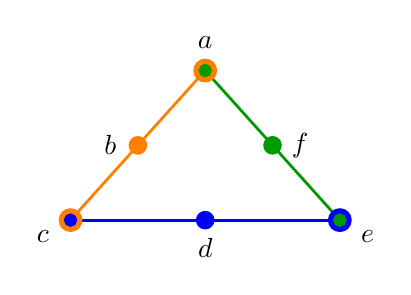
\begin{tikzpicture}[scale=0.95, every path/.style={line width=1pt}]

% coordinates
\coordinate (A) at (1.8,2.0);
\coordinate (B) at (0.9,1.0);
\coordinate (C) at (0,0);
\coordinate (D) at (1.8,0);
\coordinate (E) at (3.6,0);
\coordinate (F) at (2.7,1.0);

% contexts
\draw[orange] (A)--(B)--(C);
\draw[blue]   (C)--(D)--(E);
\draw[green!60!black] (E)--(F)--(A);

% shared atoms
\filldraw[fill=orange, draw=orange] (A) circle (4pt);
\filldraw[fill=green!60!black, draw=green!60!black] (A) circle (2pt);
\node[yshift=10pt] at (A) {$a$};

\filldraw[fill=orange, draw=orange] (C) circle (4pt);
\filldraw[fill=blue, draw=blue] (C) circle (2pt);
\node[xshift=-10pt,yshift=-6pt] at (C) {$c$};

\filldraw[fill=blue, draw=blue] (E) circle (4pt);
\filldraw[fill=green!60!black, draw=green!60!black] (E) circle (2pt);
\node[xshift=10pt,yshift=-6pt] at (E) {$e$};

% context-specific atoms
\filldraw[fill=orange, draw=orange] (B) circle (3pt);
\node[xshift=-10pt] at (B) {$b$};

\filldraw[fill=blue, draw=blue] (D) circle (3pt);
\node[yshift=-10pt] at (D) {$d$};

\filldraw[fill=green!60!black, draw=green!60!black] (F) circle (3pt);
\node[xshift=10pt] at (F) {$f$};

\end{tikzpicture}
&
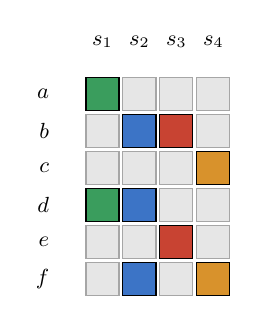
\begin{tikzpicture}[scale=0.88, transform shape]
\matrix (u) [matrix of nodes,
  nodes in empty cells,
  row sep=1pt,
  column sep=1pt,
  ampersand replacement=\&] {
|[tileone]| \& |[tilefalse]| \& |[tilefalse]| \& |[tilefalse]| \\
|[tilefalse]| \& |[tiletwo]| \& |[tilethree]| \& |[tilefalse]| \\
|[tilefalse]| \& |[tilefalse]| \& |[tilefalse]| \& |[tilefour]| \\
|[tileone]| \& |[tiletwo]| \& |[tilefalse]| \& |[tilefalse]| \\
|[tilefalse]| \& |[tilefalse]| \& |[tilethree]| \& |[tilefalse]| \\
|[tilefalse]| \& |[tiletwo]| \& |[tilefalse]| \& |[tilefour]| \\
};

\node[left=4mm of u-1-1] {\small \(a\)};
\node[left=4mm of u-2-1] {\small \(b\)};
\node[left=4mm of u-3-1] {\small \(c\)};
\node[left=4mm of u-4-1] {\small \(d\)};
\node[left=4mm of u-5-1] {\small \(e\)};
\node[left=4mm of u-6-1] {\small \(f\)};

\node[above=3mm of u-1-1] {\small \(s_1\)};
\node[above=3mm of u-1-2] {\small \(s_2\)};
\node[above=3mm of u-1-3] {\small \(s_3\)};
\node[above=3mm of u-1-4] {\small \(s_4\)};
\end{tikzpicture}
&
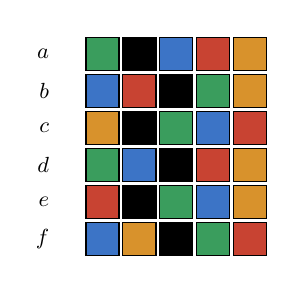
\begin{tikzpicture}[scale=0.88, transform shape]
\matrix (t) [matrix of nodes,
  nodes in empty cells,
  row sep=1pt,
  column sep=1pt,
  ampersand replacement=\&] {
|[tileone]| \& |[tilesep]| \& |[tiletwo]| \& |[tilethree]| \& |[tilefour]| \\
|[tiletwo]| \& |[tilethree]| \& |[tilesep]| \& |[tileone]| \& |[tilefour]| \\
|[tilefour]| \& |[tilesep]| \& |[tileone]| \& |[tiletwo]| \& |[tilethree]| \\
|[tileone]| \& |[tiletwo]| \& |[tilesep]| \& |[tilethree]| \& |[tilefour]| \\
|[tilethree]| \& |[tilesep]| \& |[tileone]| \& |[tiletwo]| \& |[tilefour]| \\
|[tiletwo]| \& |[tilefour]| \& |[tilesep]| \& |[tileone]| \& |[tilethree]| \\
};

\node[left=4mm of t-1-1] {\small \(a\)};
\node[left=4mm of t-2-1] {\small \(b\)};
\node[left=4mm of t-3-1] {\small \(c\)};
\node[left=4mm of t-4-1] {\small \(d\)};
\node[left=4mm of t-5-1] {\small \(e\)};
\node[left=4mm of t-6-1] {\small \(f\)};
\end{tikzpicture}
\\
(a) & (b) & (c)
\end{tabular}
\caption{Triangle-logic generalization of the \emph{Quantum Square}. (a) Greechie-style depiction of the triangle logic associated with Eq.~\eqref{eq:trianglepartitions}. The intertwining atoms \(a\), \(c\), and \(e\) are shown by concentric circles because each belongs to two contexts. (b) Atom-state incidence schema. (c) Tile rendering obtained from the grammar in Eq.~\eqref{eq:trianglegrammar}, using four recurring state colors and a black separator between support and complement. Each row lists the states with value \(1\), then the separator, and then the states with value \(0\).}
\label{fig:triangletableau}
\end{figure*}

Compared to the V-logic, the triangle uses fewer colors across more rows. Its different support pattern changes both the recurrence of colors and the positions of the separators.



\section{Prolog realizations}

The following complete SWI-Prolog programs render state symbols as digits and the separator as \texttt{|}. Double-quoted terminals in a DCG produce character codes; \texttt{[10]} supplies a newline. The companion files contain both programs and an SVG renderer that maps their output to the palettes and tile arrangements in Figs.~\ref{fig:vlogic}(c) and~\ref{fig:triangletableau}(c).

\subsection{V-logic code}

Save Listing~\ref{lst:vlogiccomplete} as \texttt{v-logic.pl}. Load it with \lstinline!use_module('v-logic.pl', []).! and run \lstinline!v_logic:output.! The result is the typographic rendering in Fig.~\ref{fig:vlogic}(d).

\begin{figure}[tbp]
\listingtitle{lst:vlogiccomplete}{Complete V-logic program with a typographic repertoire.}
\begin{lstlisting}
% SWI-Prolog: typographic V-logic tableau.
:- module(v_logic, [v_logic//0, output/0]).

% Structural layer
v_logic --> a,b,c,d,e.
a --> s1,s2,br,s3,s4,s5,n.
b --> s3,s4,br,s1,s2,s5,n.
c --> s5,br,s1,s2,s3,s4,n.
d --> s2,s4,br,s1,s3,s5,n.
e --> s1,s3,br,s2,s4,s5,n.

% Typographic repertoire and layout
s1 --> "1".
s2 --> "2".
s3 --> "3".
s4 --> "4".
s5 --> "5".
br --> "|".
n  --> [10].

% Rendering layer
output :-
    phrase(v_logic, Codes),
    format("~s", [Codes]).
\end{lstlisting}
\end{figure}

\subsection{Triangle-logic code}

Save Listing~\ref{lst:trianglecode} as \texttt{triangle-logic.pl}. Load it with \lstinline!use_module('triangle-logic.pl', []).! and run \lstinline!triangle_logic:output.! The separate modules allow both examples to be used without mixing their row rules.

\begin{figure}[tbp]
\listingtitle{lst:trianglecode}{Complete triangle-logic program.}
\begin{lstlisting}
% SWI-Prolog: typographic Wright triangle.
:- module(triangle_logic,
          [triangle_logic//0, output/0]).

% Structural layer
triangle_logic --> a,b,c,d,e,f.
a --> s1,br,s2,s3,s4,n.
b --> s2,s3,br,s1,s4,n.
c --> s4,br,s1,s2,s3,n.
d --> s1,s2,br,s3,s4,n.
e --> s3,br,s1,s2,s4,n.
f --> s2,s4,br,s1,s3,n.

% Typographic repertoire and layout
s1 --> "1".
s2 --> "2".
s3 --> "3".
s4 --> "4".
br --> "|".
n  --> [10].

% Rendering layer
output :-
    phrase(triangle_logic, Codes),
    format("~s", [Codes]).
\end{lstlisting}
\end{figure}

For colored output, load \texttt{render-tableaux.pl} and run \texttt{render\_tableaux:render\_all.} This writes one SVG file for each example. The rendering instructions are kept in the companion file so that the structural grammars remain easy to inspect.

\section{Humanities- and design-oriented interpretation}

\subsection{Structure as score}

From a design perspective, the partition logic can be interpreted as a score. It is not yet the finished artifact, just as a musical score is not yet a performance. But it prescribes a disciplined arrangement of possibilities. The grammar derived from the logic functions as a notation of relations, recurrences, and separations.

This score-like character is important because it avoids two extremes. On the one hand, it is more rigid than unconstrained improvisation: the formal structure cannot simply be ignored. On the other hand, it is less rigid than a single finished image: many realizations remain possible. The logic therefore occupies a productive middle ground between rule and freedom.

\subsection{Structural template and sign repertoire}

A simple teaching exercise is to compare the two renderings in Fig.~\ref{fig:vlogic}, then change the palette while keeping the rows fixed. A second exercise keeps the palette fixed and changes the logical source. Such comparisons may help students distinguish structural constraints from rendering choices; their educational effectiveness remains to be evaluated.

\begin{samepage}
The same V-logic may therefore become:
\begin{itemize}
\item a colored tile image,
\item a typographic grid,
\item a sequence of syllables,
\item a rhythmic or harmonic pattern,
\item or a data-driven animation.
\end{itemize}
\end{samepage}
Beyond the visual examples presented here, a sonic prototype has been developed by Christian Jendreiko in collaboration with the composer Klaus Roeder. Further work in this direction is being pursued by a research group led by Christian Jendreiko at HSD University of Applied Sciences in D\"usseldorf. The group includes Klaus Roeder, Bj\"orn Lellmann, and Robert Eisinger.

\subsection{From diagram to perceptual offering}

In science communication, it is often tempting to regard visualization as a transparent window onto a concept. Our approach suggests a more careful view. The generated object is not a transparent copy of the logic. It is a \emph{perceptual offering}: a structured artifact that affords certain acts of recognition, comparison, and reflection.

The value of such artifacts lies partly in their legibility and partly in their sensuous force. A purely formal matrix may be clearer analytically; a more aesthetic tile arrangement may be more memorable or engaging. These are not mutually exclusive aims, but they are distinct. The tension between them should be treated as a design problem rather than suppressed.

\subsection{Complementarity without overstatement}

The V-logic permits a staged introduction to complementarity: the hypergraph shows distinct contexts and their overlap, while the state table makes the existence of global truth assignments explicit. Kochen-Specker configurations without such assignments require a further step.

The tile image can support this comparison, provided that the source contexts are shown alongside it. Whether this improves understanding is an empirical question.

\section{Discussion}

Several points deserve emphasis.

First, the construction is not limited to the V-logic. Any finite partition logic with separating two-valued states can be translated into an SGLG in the manner described above. Larger examples, including pentagon logics and more intricate pasted structures, should yield richer aesthetic and pedagogical possibilities \cite{wright,svozil-2001-eua}.

Second, not every finite quantum structure admits a separating set of two-valued states, and not every partition logic admits the kind of quantum realization given for the V-logic. The Wright triangle illustrates the latter distinction. Structures without suitable state supports would need a different translation, perhaps based on their context incidence or orthogonal representations.

Third, the distinction between logical skeleton and repertoire is not merely a convenience of notation. It is what allows one and the same source structure to appear across media and to function both as a formal object and as a generative score.

Fourth, the method invites empirical investigation. Which mappings are most understandable to non-specialist audiences? Which visual or sonic forms best communicate overlap of contexts? When does aesthetic richness enhance understanding, and when does it obscure it? These are open interdisciplinary research questions.

\section{Conclusion}

We have proposed and exemplified a concrete bridge between partition logic and Generative Logic. The bridge consists of a translation from finite partition logics with separating two-valued states into simple non-recursive grammars, together with a principled separation between formal skeleton, sign repertoire, and rendering layer.

Using the V-logic \(L_{12}\), we derived a modular visual artifact, the \emph{Quantum Square}, and a typographic rendering of the same grammar. We also gave additional formal examples, including a horizontal sum of binary partitions and a triangle-logic generalization.

The broader significance of the method is double. For design and artistic research, it opens a disciplined way of using logical structures as generative scores. For science communication, the combination of source diagrams and generated artifacts offers a way to introduce contexts and their overlap. The demonstrated result is precise: atom--state incidence can be translated into perceptible form, while the chosen states, ordering, and rendering remain explicit design decisions.

\begin{acknowledgments}
Christian Jendreiko would like to thank Fran\c{c}ois Fages, Thierry Marianne, and Guy Narboni for the invaluable insights gained during a collaborative working session in Paris.
This research was funded in whole or in part by the \textit{Austrian Science Fund (FWF)} [Grant \textit{DOI:10.55776/PIN5424624}].
The authors acknowledge TU Wien Bibliothek for financial support through its Open Access Funding Programme.
\end{acknowledgments}

\bibliography{svozil}

\end{document}
